\chapter{Introduction}\label{chap:introduction}
\section{Overview}
The field of Topological Data Analysis (TDA) uses tools from topology and algebraic topology to rigorously study the shape (e.g. clusters, loop, tendrils, modes, ridges) of point cloud data and functional data.
In recent years the field of TDA has been advancing rapidly, resulting in many theoretical developments as well as applications (see \cite{giuntiLazovskis} for an online database of applications of TDA, \cite{rabadanBlumberg_2019} for applications to biology and \cite{hensel_2021} for applications to machine learning, to name a few).
\begin{figure}[h]
  \centering
  \begin{subfigure}{0.7\textwidth}
    \centering
    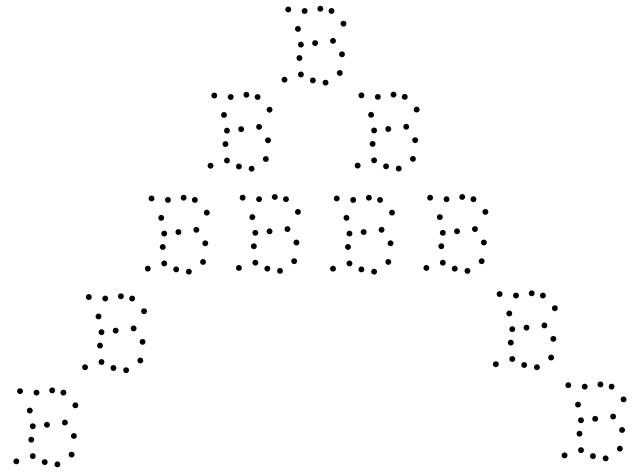
\includegraphics[width=0.5\linewidth]{./figures/exampel-dataset.png}
    \caption{}
  \end{subfigure}
  \begin{subfigure}{0.7\textwidth}
    \centering
    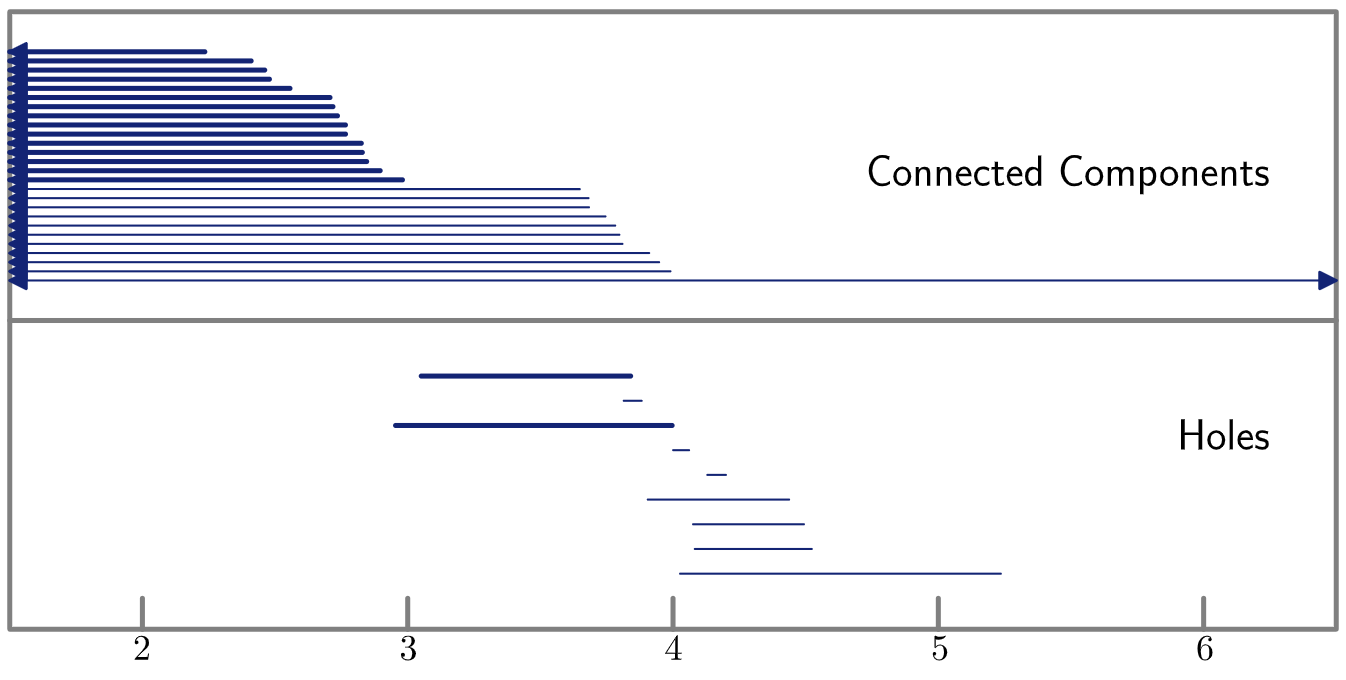
\includegraphics[width=0.7\linewidth]{./figures/example-barcode.png}
    \caption{}
  \end{subfigure}
  \caption{An example of a data set (a) and its barcode (b). The function used to produce the level sets is the distance function to our dataset. The horizontal line represents geometric scale with logarithmic graduation. Taken from \cite{oudot_2015}.}
  \label{fig:barcode-example}
\end{figure}

In general, the workflow of TDA relies on constructing a \textdef{filtration} $F(X)$ (i.e. a commutative diagram of topological spaces) which somehow encodes information about the shape of a data set $X\subset\Rb^n$, and then analyzing the structure of $F(X)$ using techniques from topology and algebraic topology \cite{botnanLesnick_2022}.
The most widely used instance of this workflow is when indexing $F(X)$ by a totally ordered set (e.g. $\Rb$ or $\Nb$).
If we wish to emphasize that a filtration is indexed by a totally ordered set, we will call it a \textdef{1-parameter filtration}.
The construction of a filtration can take many forms depending on the type of data and the kind of questions one is interested in, but a typical example is the \textdef{offset filtration}:
for each $t\in\Rb$, let $X_t=d_X^{-1}((-\infty, t])$ where $d_X\colon \Rb^n\to [0,\infty), y\mapsto\inf_{x\in X}\norm{x-y}$.
Then the offset filtration $\offset(X)$ is the collection of all $X_t$ together with the inclusion maps $s\leq t\iff X_s\hookrightarrow X_t$.
Note that $\offset$ is a functor from the poset $\Rb$ to $\Top$, the category of topological spaces.
We can then apply the $i$-th homology functor with coefficients in a field $\field$ to $\offset(X)$ to get a collection $H_i(X)$ of $\field$-vector spaces $H_i(X_t), t\in\Rb$ together with linear map induced by the inclusions.
The composition of $\offset$ and the $i$-homology gives a functor from $\Rb$ to $\Vect$, the category of $\field$-vector spaces. We will see in Chapter \ref{chap:persistenceModules} that this is an example of a (1-parameter) persistence module over $\Rb$.
There is a structure theorem \cite{BotnanCrawley_2018} that tells us that we can always decompose such a collection of vector spaces into direct sum of \textdef{interval modules}, i.e. an indicator module supported on an interval.
These, in a sense, encode the persistence of $i$-th dimensional hole in our data set across the filtration - long intervals correspond to "true" features.
The collection of all such intervals is called the \textdef{barcode} of $X$.
In Figure \ref{fig:barcode-example} we have example of a data set together with the $H_0$ and $H_1$ barcodes.
In the top barcode, the 11 lines correspond to the 11 B's which merge to form the big A around $4$, which then persists as a single cluster. 
Also note the line from 4 until a little over 5 in the bottom barcode, corresponding to the loop in the top part of the A.
For more details on algorithms used to compute barcodes, see \cite{oudot_2015,deyWang_2022}.
This process of constructing a 1-parameter filtration, applying homology to get a 1-parameter persistence module and then computing its decomposition to obtain the barcode is called \textdef{(1-parameter) persistent homology}.
\begin{figure}[h]
  \centering
  \begin{subfigure}{.45\textwidth}
    \centering
    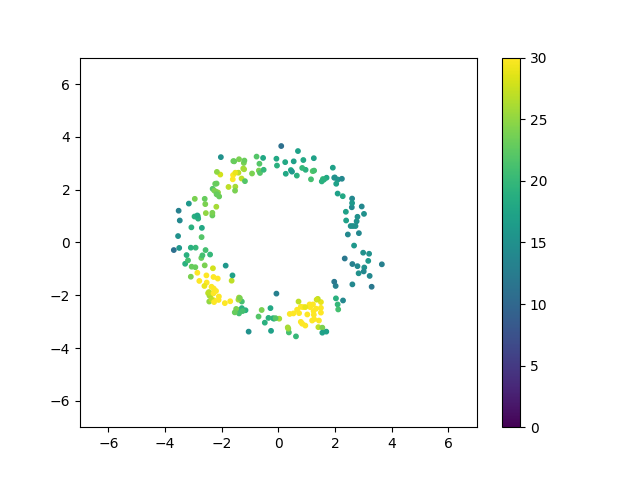
\includegraphics[width=.9\linewidth]{./figures/circle}
    \caption{}
    \label{fig:circle}
  \end{subfigure}%
  \begin{subfigure}{.45\textwidth}
    \centering
    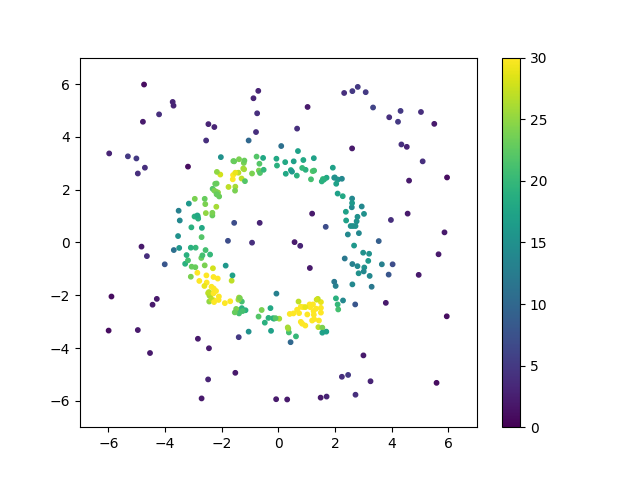
\includegraphics[width=.9\linewidth]{./figures/circle-all-points}
    \caption{}
    \label{fig:circle-all-points}
  \end{subfigure}
  \begin{subfigure}{.45\textwidth}
    \centering
    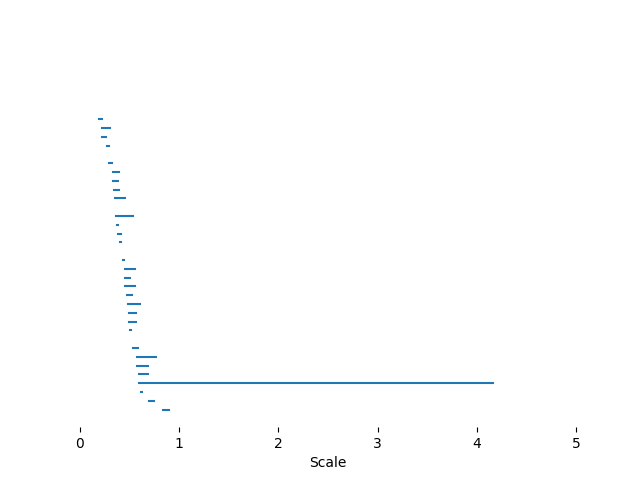
\includegraphics[width=.9\linewidth]{./figures/barcode-circle}
    \caption{}
    \label{fig:barcode-circle}
  \end{subfigure}%
  \begin{subfigure}{.45\textwidth}
    \centering
    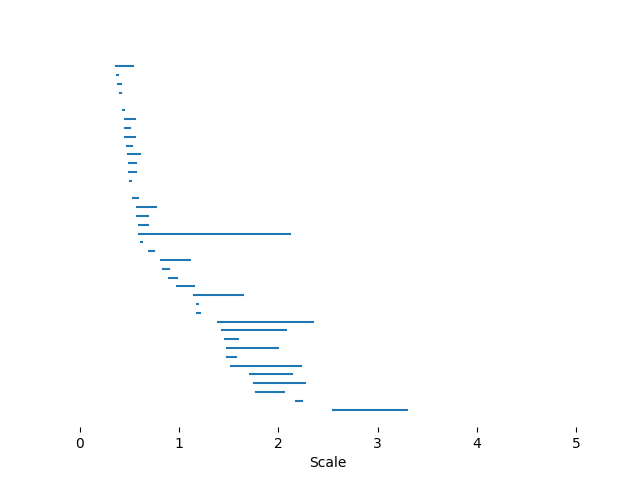
\includegraphics[width=.9\linewidth]{./figures/barcode-all-points}
    \caption{}
    \label{fig:barcode-all}
  \end{subfigure}
  \caption{
    \textbf{(a)} Circular data set colorized by local density estimate.
    \textbf{(b)} Data set from (a) with added noise.
    \textbf{(c)} The $H_1$ barcode of the data in (a).
    \textbf{(d)} The $H_1$ barcode of the data in (b).
    Taken from \cite[section 3.4]{botnanLesnick_2022}}
  \label{fig:circles-full}
\end{figure}

However, in \cite[Section 4]{BulmbergEtal_2012} it was shown that 1-parameter persistent homology is fragile.
In other words, an addition of small amount of noise can drastically change the barcode.
See for example Figure \ref{fig:circles-full}: while the $H_1$ barcode of the "clean" data set clearly captures the circular shape of the data, this is completely lost in the barcode of the noisy data.
A solution to this (and other) problems is to consider a filtration indexed by two parameters: scale (as in the offset filtration) and density threshold. This is called a \textdef{bi-filtration} or a \textdef{multi-filtration}.
A multi-filtration, instead of being a functor from a totally ordered set to $\Top$ is a functor from $P$ to $\Top$, where $P$ could be a finite product of totally ordered sets (e.g. $\Nb^2, \Rb^n$, where the partial ordering is given by $(x_i)_i\leq (y_i)_i\iff x_i\leq y_i$ for all $i$) or a different poset altogether. 
Given a multi-filtration, we can again apply homology with coefficients in a field $\field$ to obtain a multi-parameter persistence module, but unfortunately there is no decomposition similar to the barcode in the 1-parameter case \cite{gunnarAfra_2007}.
For more details regarding multi-parameter persistence and possible alternatives to the barcode see \cite{botnanLesnick_2022,botnan_2021}.
The aim of this paper is to prove the following decomposition theorem.
\begin{theorem}\label{theorem:main}
  Let $\category$ be any small category and $M\colon\category\to\Vect$ a pointwise finite dimensional (pfd) persistence module.
  Then $M$ has an essentially unique decomposition into indecomposable persistence modules.
\end{theorem}
Therefore,
\section{Outline}
In Chapter \ref{chap:persistenceModules}, we start by defining persistence modules as well as some elementary notions such as direct sum, kernels and submodules. 
We then prove that persistence modules are indeed modules over a certain algebra, and construct a tensor product.
This is followed by defining a hom functor which is right adjoint to the tensor product and proving the tensor-hom adjunction.

In Chapter \ref{chap:existence} we define the notions of pure and pure-injective modules. 
These are then used, together with the tensor-hom adjunction to prove that every pfd persistence module is pure-injective (Lemma \ref{lemma:PRepsArePure}).
This property, together with the fact that a direct summand is a pure submodule and the union of a chain of pure submodules is pure (Lemmas \ref{lemma:directSumIsPure} and \ref{lemma:unionIsPure} respectively) are the key to the proof of Lemma \ref{lemma:indecomposableSummand}, which states that every pfd persistence module has an indecomposable summand.
It is then straightforward to prove that every pfd persistence module is a direct sum of indecomposables (Theorem \ref{thm:indecomposableDecomposition}).
I would like to thank William Crawley-Boevey who shared the outline for this chapter, as well as the proof of Lemma \ref{lemma:PRepsArePure}, with Magnus Botnan which then shared them with me.

Chapter 4 starts by proving that a pfd persistence module is indecomposable if and only if it has a local endomorphism ring, which is done by a pointwise application of Fitting's Lemma, analogous to paragraphs two to five in \cite[Section 3]{BotnanCrawley_2018}.
This is then used to adapt the proof of the Krull-Remak-Schmidt-Azumaya theorem from \cite[Section 5.1]{popescu_1973}, which proves that the decomposition of a pfd persistence module into indecomposable summands is essentially unique.